\documentclass[tikz, border=10pt]{standalone}
\usepackage{varwidth}
\usetikzlibrary{backgrounds}
\begin{document}
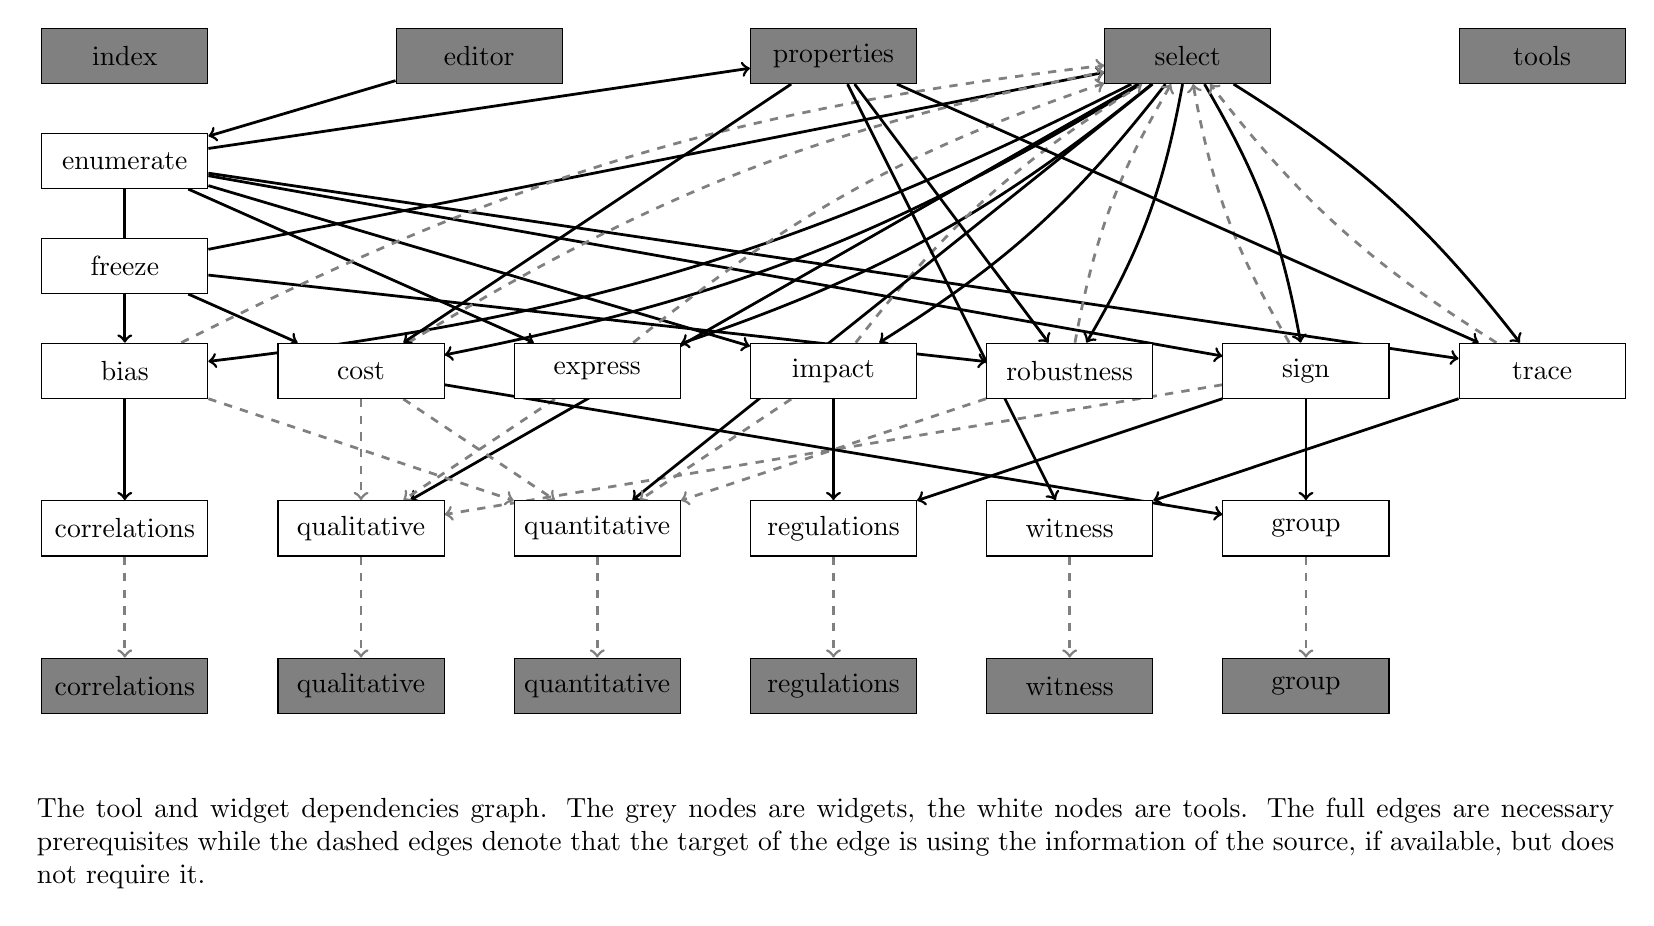
\begin{tikzpicture}
\tikzstyle{widget}=[draw,
fill=gray,
rectangle, 
minimum width=60pt,
minimum height=20pt] 
\tikzstyle{tool}=[draw, fill=white, rectangle, minimum width=60pt, minimum height=20pt]  
\tikzstyle{tool}=[draw, fill=white, rectangle, minimum width=60pt, minimum height=20pt]  
\tikzstyle{must} = [->, solid, line width=1pt]
\tikzstyle{may} = [->, dashed, line width=1pt, gray]
	\node[widget] (index) at (0,0) {index};
	\node[widget] (editor) at (4.5,0) {editor};
	\node[widget] (properties) at (9,0) {properties};
	\node[widget] (select) at (13.5,0) {select};
	\node[widget] (tools) at (18,0) {tools};

	\node[tool] (enumerate) at (0,-1.333) {enumerate};
	
	\node[tool] (freeze) at (0,-2.666) {freeze};
  
	\node[tool] (bias) at (0,-4) {bias};
	\node[tool] (cost) at (3,-4) {cost};
	\node[tool] (express) at (6,-4) {express};
	\node[tool] (impact) at (9,-4) {impact};
	\node[tool] (robustness) at (12,-4) {robustness};
	\node[tool] (sign) at (15,-4) {sign};
	\node[tool] (trace) at (18,-4) {trace};
  
  	\node[tool] (correlations) at (0,-6) {correlations};
	\node[tool] (qualitative) at (3,-6) {qualitative};
	\node[tool] (quantitative) at (6,-6) {quantitative};
	\node[tool] (regulations) at (9,-6) {regulations};
	\node[tool] (witness) at (12,-6) {witness};
	\node[tool] (group) at (15,-6) {group};
	
	\node[widget] (correlations_w) at (0,-8) {correlations};
	\node[widget] (qualitative_w) at (3,-8) {qualitative};
	\node[widget] (quantitative_w) at (6,-8) {quantitative};
	\node[widget] (regulations_w) at (9,-8) {regulations};
	\node[widget] (witness_w) at (12,-8) {witness};
	\node[widget] (group_w) at (15,-8) {group};
	
	
	\begin{scope}[on background layer]
	\draw[must] (editor) to (enumerate);
	
	
	\draw[must] (enumerate) to (properties);
	
	\draw[must] (enumerate) to (bias);
	\draw[must] (enumerate) to (express);
	\draw[must] (enumerate) to (impact);
	\draw[must] (enumerate) to (sign);
	\draw[must] (enumerate) to (trace);	
	

	\draw[must] (freeze) to (select);	
	\draw[must] (freeze) to (cost);
	\draw[must] (freeze) to (robustness);
	
	\draw[must, bend left=10] (select) to (bias);
	\draw[must, bend left=10] (select) to (cost);
	\draw[must, bend left=10] (select) to (express);
	\draw[must, bend left=10] (select) to (impact);
	\draw[must, bend left=10] (select) to (robustness);
	\draw[must, bend left=10] (select) to (sign);
	\draw[must, bend left=10] (select) to (trace);
	
	\draw[may, bend left=10] (bias) to (select);
	\draw[may, bend left=10] (cost) to (select);
	\draw[may, bend left=10] (express) to (select);
	\draw[may, bend left=10] (impact) to (select);
	\draw[may, bend left=10] (robustness) to (select);
	\draw[may, bend left=10] (sign) to (select);
	\draw[may, bend left=10] (trace) to (select);
	
	\draw[must] (bias) to (correlations);

	\draw[must] (properties) to (cost);
	\draw[must] (properties) to (robustness);
	\draw[must] (properties) to (trace);
	
	\draw[must] (select) to (qualitative);
	\draw[may] (cost) to (qualitative);
	\draw[may] (express) to (qualitative);
	\draw[may] (sign) to (qualitative);
	
	\draw[must] (select) to (quantitative);
	\draw[may] (bias) to (quantitative);
	\draw[may] (cost) to (quantitative);
	\draw[may] (impact) to (quantitative);
	\draw[may] (robustness) to (quantitative);
	
	\draw[must] (impact) to (regulations);
	\draw[must] (sign) to (regulations);
	
	\draw[must] (trace) to (witness);
	\draw[must] (properties) to (witness);
	
	\draw[must] (cost) to (group);
	\draw[must] (sign) to (group);
	
	\draw[may] (correlations) to (correlations_w);
	\draw[may] (qualitative) to (qualitative_w);
	\draw[may] (quantitative) to (quantitative_w);
	\draw[may] (regulations) to (regulations_w);
	\draw[may] (witness) to (witness_w);
	\draw[may] (group) to (group_w);
	\end{scope}

	\node[] (desc) at (8.9,-10) {
	\begin{varwidth}{570pt}The tool and widget dependencies graph. The grey nodes are widgets, the white nodes are tools. The full edges are necessary prerequisites while the dashed edges denote that the target of the edge is using the information of the source, if available, but does not require it.
	\end{varwidth}	
	};
\end{tikzpicture}
\end{document}